In this section we document the main shape variations we include in the 
2D ($m_{ll}, m_T$) analysis performed in the low mass analysis of the 0-Jet bin. 
Figure~\ref{fig:qqww_shapevar_theory}-\ref{fig:top_shapevar_theory} 
show the shape systematics for the main backgrounds $qq\to WW$, $W$+Jets and Top. 
Figure~\ref{fig:qqww_shapevar_instr} show the shape systematics due to the 
intrumental uncertainties in the physics objects reconstruction using 
$qq\to WW$ process as an example. Note that we include all the instrumental 
uncertainties induced shape systematics for all processes where the central shapes 
are taken from simulation. More detailed description can be found in Reference~\cite{MVASyst}. 

%%%%%%%%%%%%%%%%%%%%%%%%%%%%%%%
\begin{figure}[!hbtp]
\centering
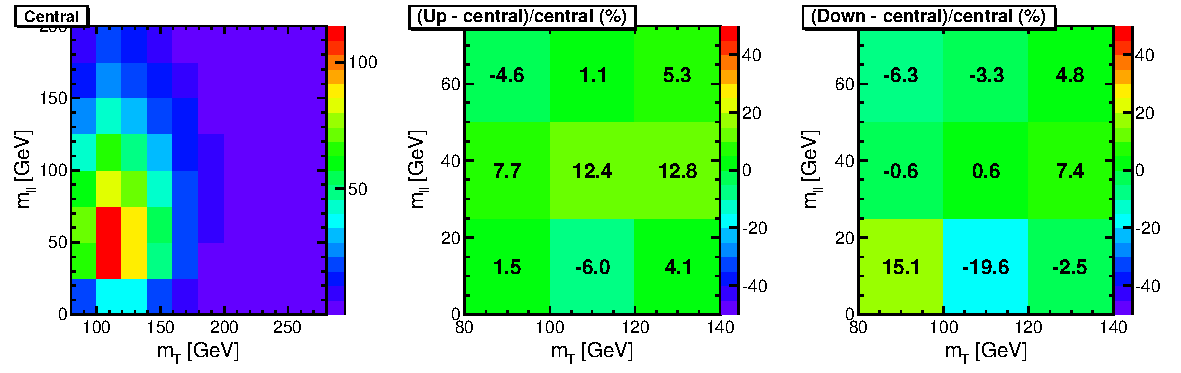
\includegraphics[width=1.0\textwidth]{figures/qqWW_WWNLOBounding_2D_mH125_0j_of.pdf}
\caption{ The shape variations for the $qq\to WW$ process due to higher order 
theoretical uncertainties. }
\label{fig:qqww_shapevar_theory}
\end{figure}
%%%%%%%%%%%%%%%%%%%%%%%%%%%%%%%

%%%%%%%%%%%%%%%%%%%%%%%%%%%%%%%
\begin{figure}[!hbtp]
\centering
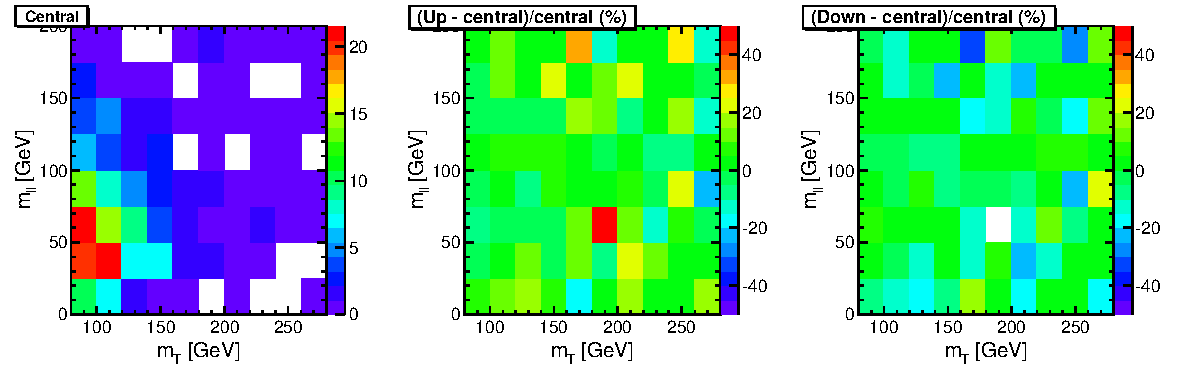
\includegraphics[width=1.0\textwidth]{figures/Wjets_WBounding_2D_mH125_0j_of.pdf}
\caption{ The shape variations for the $W$+jets process due to the fake rate uncertainties in data. }
\label{fig:wjets_shapevar_theory}
\end{figure}
%%%%%%%%%%%%%%%%%%%%%%%%%%%%%%%


%%%%%%%%%%%%%%%%%%%%%%%%%%%%%%%
\begin{figure}[!hbtp]
\centering
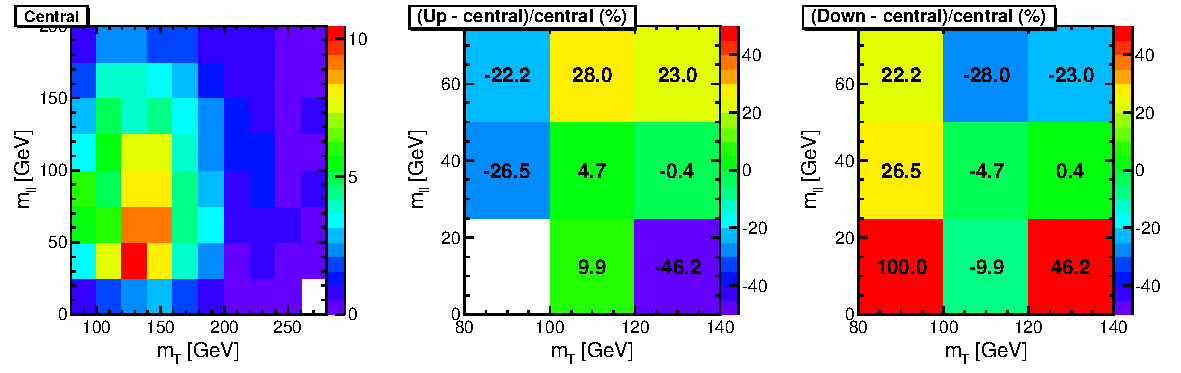
\includegraphics[width=1.0\textwidth]{figures/Top_TopBounding_2D_mH125_0j_of.pdf}
\caption{ The shape variations for the Top process due to higher order theoretical uncertainties.}
\label{fig:top_shapevar_theory}
\end{figure}
%%%%%%%%%%%%%%%%%%%%%%%%%%%%%%%


%%%%%%%%%%%%%%%%%%%%%%%%%%%%%%%
\begin{figure}[!hbtp]
\centering
\subfigure[Lepton Momentum Resolution]{
\label{subfig:lepres}
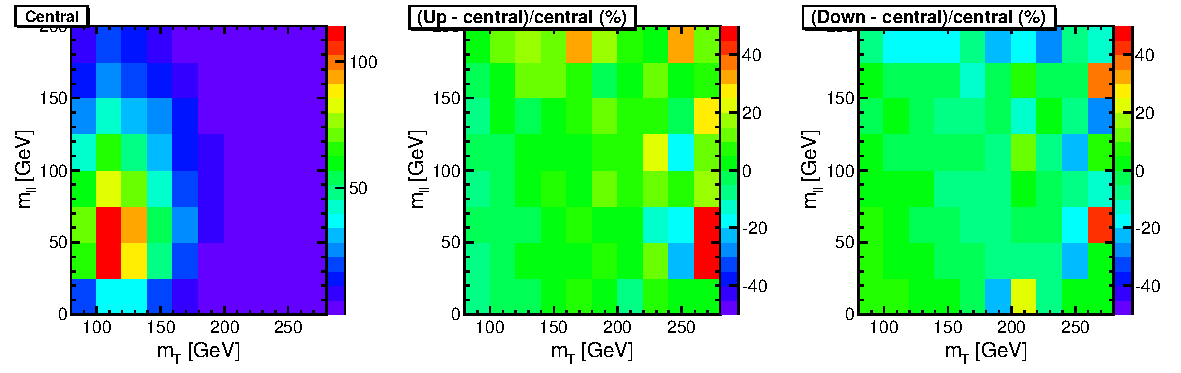
\includegraphics[width=1.0\textwidth]{figures/qqWW_LepResBounding_2D_mH125_0j_of.pdf}
}
\subfigure[Lepton Efficency]{
\label{subfig:lepres}
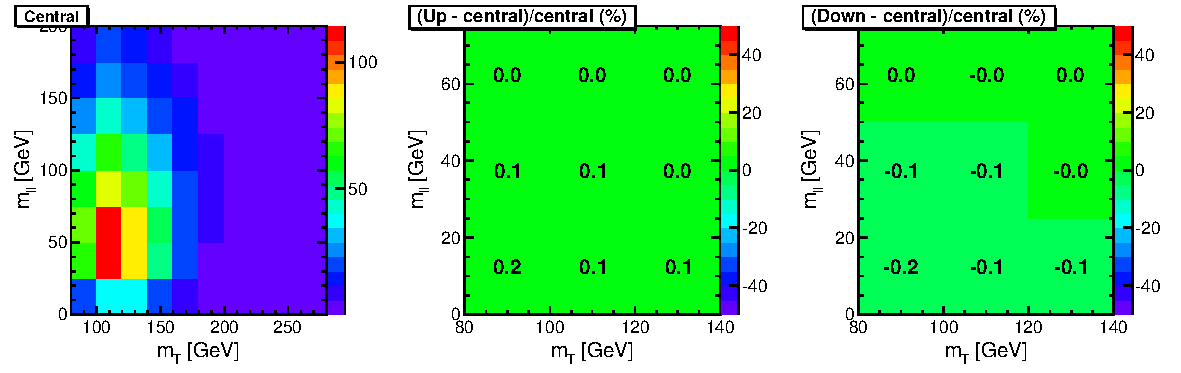
\includegraphics[width=1.0\textwidth]{figures/qqWW_LepEffBounding_2D_mH125_0j_of.pdf}
}
\subfigure[\met\ Resolution]{
\label{subfig:lepres}
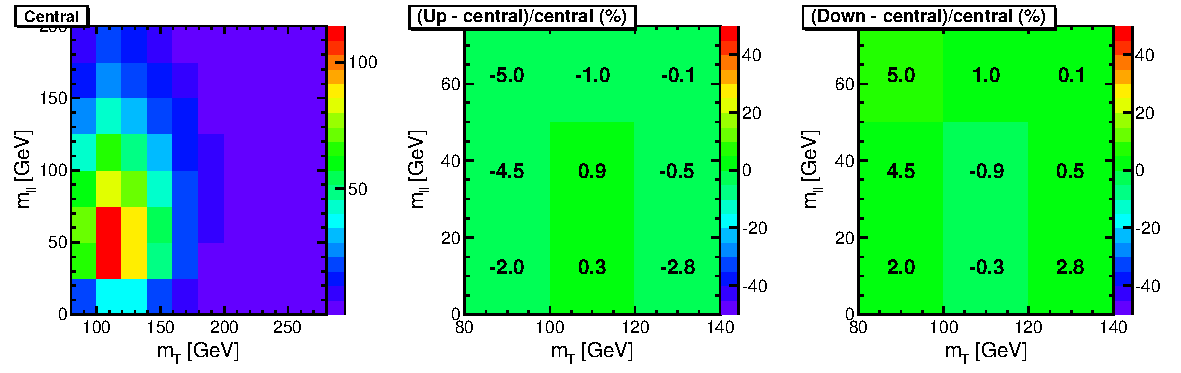
\includegraphics[width=1.0\textwidth]{figures/qqWW_METResBounding_2D_mH125_0j_of.pdf}
}
\subfigure[JET Enery Scale]{
\label{subfig:lepres}
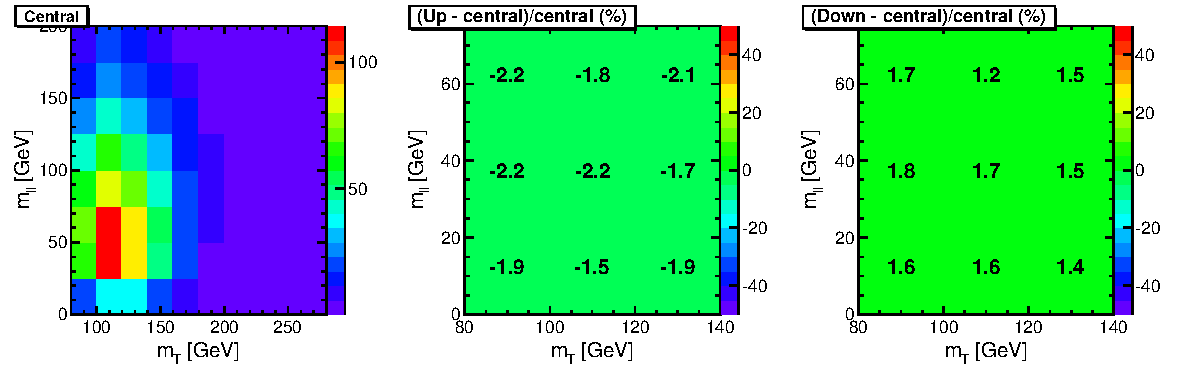
\includegraphics[width=1.0\textwidth]{figures/qqWW_JESBounding_2D_mH125_0j_of.pdf}
}
\caption{ The shape variations for the $qq\to WW$ process due to instrumental uncertainties on the 
physics objects reconstruction. }
\label{fig:qqww_shapevar_instr}
\end{figure}
%%%%%%%%%%%%%%%%%%%%%%%%%%%%%%%

